Cantidades como la densidad de estados, la densidad de carga entre otras requieren de integrales sobre el espacio rec\'iproco.

\begin{equation}
    \bar{A} = \int _{BZ} A(k) d(k)
\end{equation}

\noindent Para que la integral sea evaluada computacionalmente debe ser discretizada mediante una sumatoria de pesos que se asignan a los puntos del espacio rec\'iproco.

\begin{equation}
    \int _{BZ} d(k) \to \sum _{K} w_{K}
\end{equation}

\noindent A continuaci\'on se da un ejemplo con una grilla de $4 \times 4$.

\begin{figure}[H]
    \centering
    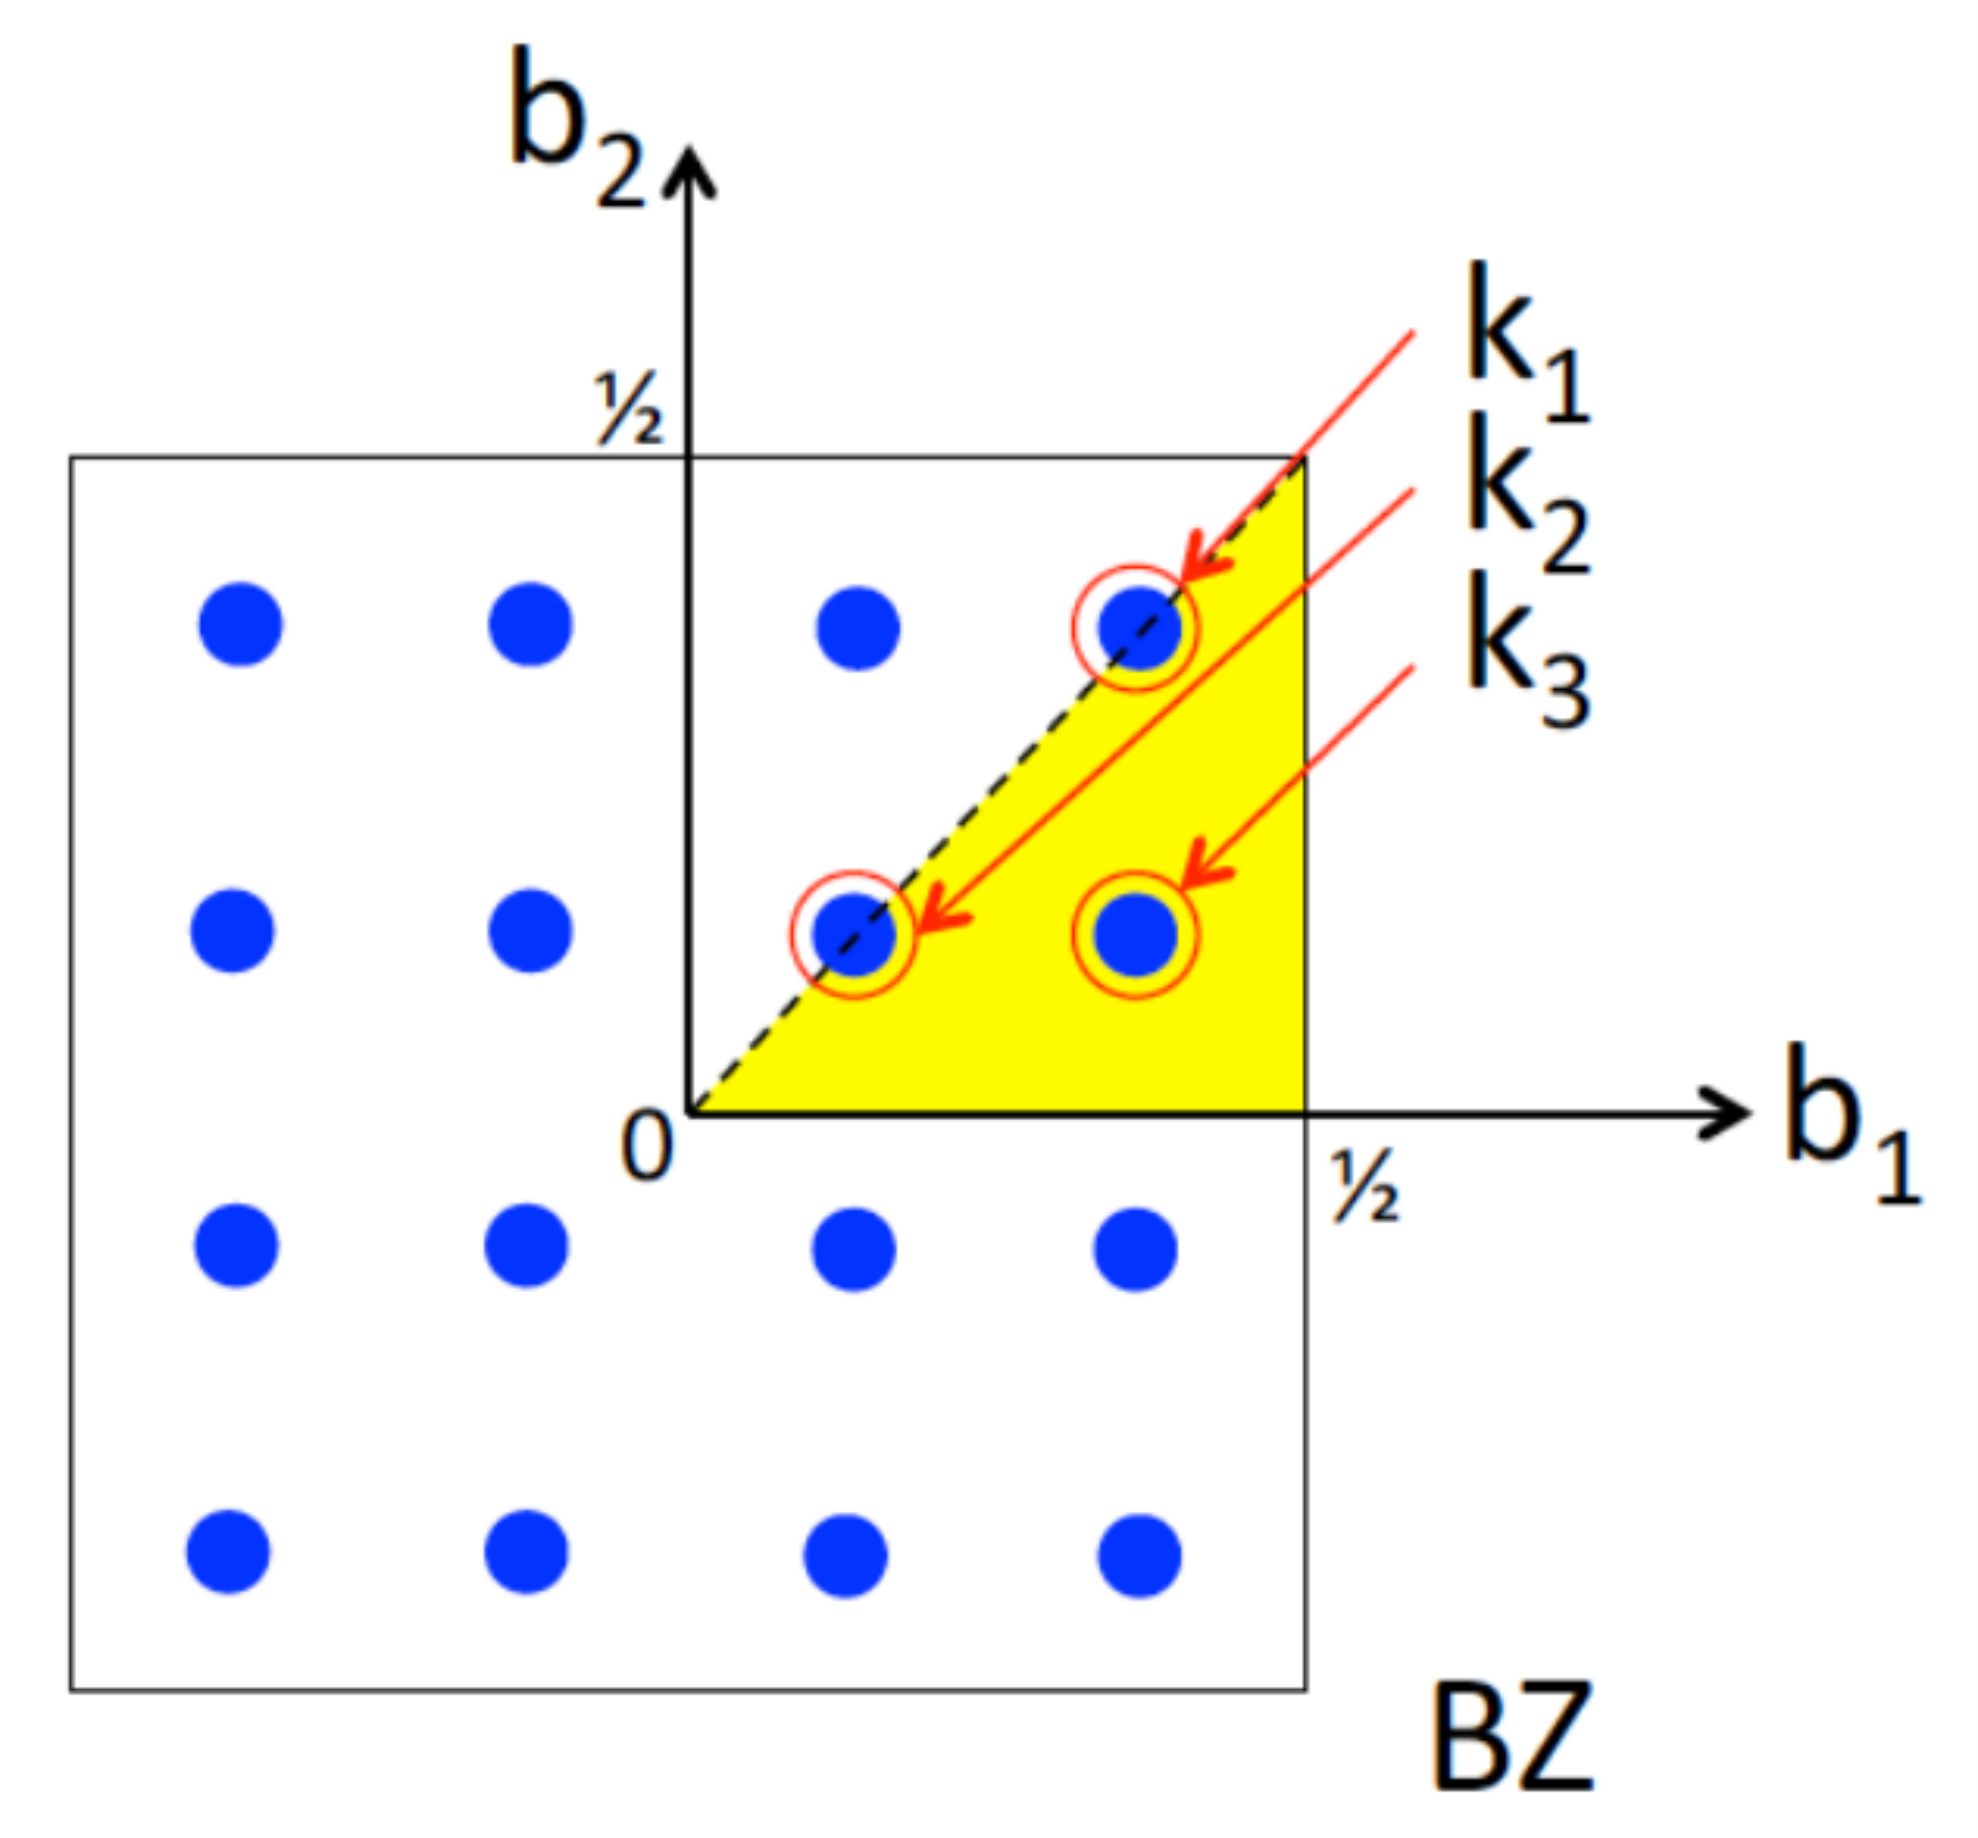
\includegraphics[width=0.6\linewidth]{contenido/calculos_computacionales/integrales_reciproco/img_reciproco/ZonaBrillouin}
\end{figure}

\noindent los pesos correspondientes son los siguientes.

\begin{eqnarray}
4 \times K_{1} \to w_{1} = \frac{4}{16} = \frac{1}{4} \nonumber \\
4 \times K_{2} \to w_{2} = \frac{4}{16} = \frac{1}{4}  \\
8 \times K_{3} \to w_{1} = \frac{8}{16} = \frac{1}{2} \nonumber
\end{eqnarray}

\noindent la integral discretizada seria la siguiente

\begin{equation}
    \int _{BZ} A(k) d(k) \approx \frac{1}{4}A(K_{1}) + \frac{1}{4}A(K_{2}) + \frac{1}{2}A(K_{3})
\end{equation}
